\documentclass[twocolumn,10pt]{IEEEtran}

\usepackage{wrcecapstone}
\newcommand{\myroot}{.}
\hypersetup{%
	pdfauthor={Corwin Stites},
	pdftitle={Unmanned underwater vehicle mobile mesh networks: applications for hydrographic surveying},
	pdfsubject={weapons, robotics, and control engineering},
	pdfkeywords={UUV, mesh networks, hydrographic survey}}
\bibliographystyle{IEEEtran}
\usepackage{cite}
\usepackage{tabularx}

% Fall Smester Bowman Research Report
\title{Unmanned underwater vehicle mobile mesh networks: applications for hydrographic surveying}
\author{MIDN 1/C Corwin W. Stites\thanks{Author is with the Department of Weapons, Robotics, and Control Engineering at the United States Naval Academy. Address for correspondence: \emph{m216468@usna.edu}}}
\date{December 3, 2020}

% for EW495 title page?
\usepackage{wrcetitlepage}
\coursenumber{EW495}
\student{MIDN 1/C C. Stites}
\advisor{Assistant Professor D. Evangelista}
%\coverpicture{\includegraphics[height=1.88in]{\myroot/figures/problem-statement-1a.png}}

\begin{document}
%\maketitlepage
\maketitle

\begin{abstract}
Underwater surveying is a costly and time consuming endeavor. My project is investigating how a mobile mesh network could be applied to make hydrographic surveys more efficient and accurate. Such a network would consist of a group of sonar equipped Unmanned Underwater Vehicles (UUVs) connected via a mesh network actuated through an acoustic modem. The project focus is on the spatial arrangement of the nodes as well as how nodes of the mesh network would communicate for best effect to accomplish fast hydrographic surveying of a predetermined area or fast location of an underwater target of interest.  
\end{abstract}

\begin{IEEEkeywords}
UUV, mesh networks, hydrographic survey, swarms
\end{IEEEkeywords}

\section{Introduction}
Nearly 80\% of U.S. international trade moves through ports which require constant bathymetry to ensure the safe transit of vessels. Underwater surveying is critical to detecting changing conditions or obstructions that could be hazardous to navigation. 500,000 square miles of U.S. waters are deemed navigationally significant and must be regularly surveyed by the National Oceanic and Atmospheric Administration (NOAA). These surveys are typically carried out by a single ship or underwater vehicle operating in a search pattern. This process requires a large amount of time and resources and as a result the NOAA must prioritize which areas it surveys \cite{noaa2009hydrographic}.
	
The disappearance of Malaysia Airline Flight 370 in March of 2014 further illustrated the lack of surveying capabilities for large areas of ocean. Over 200,000 square kilometers were searched in two separate operations in an unsuccessful attempt to find the missing aircraft \cite{australia2018joint}. Another revelation from the search for MA 307 was the validation of UUV fleet technology. The company Ocean Infinity used its fleet of eight advanced surveying UUVs for the first time on a large scale. The fleet was able to search in a collaborative pattern, surveying areas much more quickly and efficiently than any other search asset \cite{economist2018fantastical}. This new application of fleet technology showed that UUV fleets prove more robust and efficient at surveying large areas. The individual bots in the fleet, while mostly autonomous, still required their search paths to be set by humans and still required periodic communication with the main ship via an acoustic modem \cite{haun2017ocean}. 	

There are possibilities to further streamline a fleet UUV system. Removing the need for operator route planning and ship communication would add an additional element of autonomy. This would be useful for operators trying to expand the size of a UUV fleet or trying to operate multiple fleets simultaneously. More numerous and larger fleets capable of being operated from one manned element would allow for even greater capabilities in searching for deep water objects and carrying out routine hydrographic surveying. A mesh network is a network in which individual assets in the group (called nodes) can communicate with each other cooperatively to function independent of outside control. Utilization of a mesh network could allow for these developments. With a mesh control algorithm, routes would not need to be planned by human operators. A search area could merely be given to the fleet and the mesh protocol could then plan the search patterns of individual assets. Furthermore, the mesh protocol could correct the course errors of individual assets via relative position to other nodes when a particular node’s dead reckoning goes off course. This means guidance from the ship would not be required. For this model, knowledge of predetermined UUV tasks would have to be built into each node to limit the information transmitted between nodes. 



\subsection{Mesh network architectures for efficient and reliable hydrographic survey}

An enabling factor for using networked UUVs for efficient hydrographic survey is to find network architectures which are robust and reliable in the face of disruptions. Architectural decisions which I hope to examine include algorithms for routing messages between nodes, and for reconfiguring around network gaps. Within these, there are various costs associated with routing of single packets versus flooding \cite{zahn2009empirical}, message routing based on link quality \cite{hamraz2019wireless}, and methods of re-routing and self-healing the network when a UUV node is lost \cite{trehan2019algorithms}. 

To help choose between these various network architecture design alternatives, here I develop a tool to simulate two aspects (which I term ``survivability rate'' and ``surving path length'', discussed below) in intact and damaged mesh networks of various topologies. For these initial steps, I used the \lstinline{networkx} library \cite{hagberg2008exploring, sphyce2015networkx} in Python 3.7 (example shown in \fref{fig:2}).  This portion of the project was important for laying the groundwork of developing methods for building and testing networks in a coding environment in order to begin further exploring more advanced topics like healing algorithms, network throughput, and data rates next semester. 
\begin{figure}[h]
\begin{center}
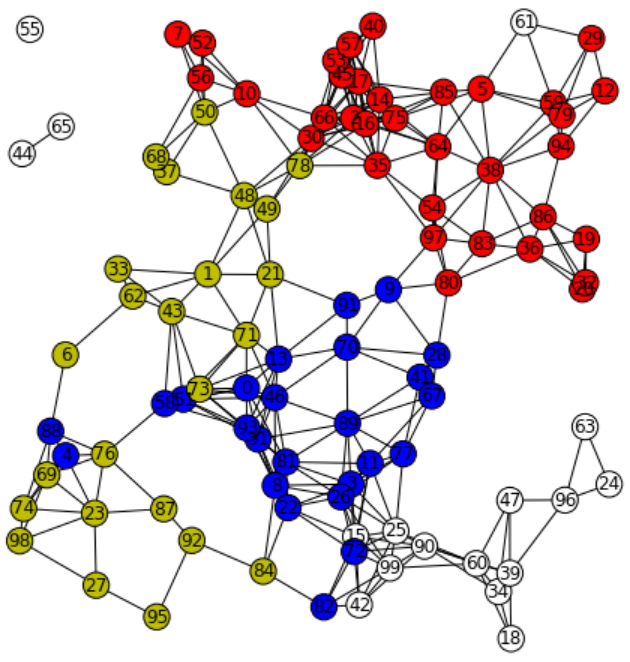
\includegraphics[width=0.33\columnwidth]{figures/fig1.png}
\end{center}
\caption{An example of a flooding algorithm being tested with the Python \lstinline{networkx} library. The graphic displays three different spreading patterns from various starting nodes according to a flooding algorithm. A simulation like this would be used to test relevant metrics of network architectures \cite{sphyce2015networkx}.}
\label{fig:2}
\end{figure}

The networks discussed in this paper are abstractions in which I consider a spatial arrangement within a \SI{40x40}{\meter} grid and transport delays consistent with the speed of sound in water ($c=\SI{1500}{\meter\per\second}$). As the work progresses, the simulations will be revised as appropriate to model underwater acoustic hardware, e.g. \fref{tab:1}.
\begin{table}[h]
\caption{Specifications for an ARM9 Cortex-M3 acoustic modem. The network architecture will have to be designed around the data rates both transmitting and receiving for an underwater system such as this \cite{arm2013acoustic}.}
\label{tab:1}
\begin{center}
\begin{tabular}{ll}
  \toprule
  feature & description \\
  \midrule
  MCU & ARM9 (Cortex-M3) \\
  resonant frequency & \SI{70}{\kilo\hertz} \\
  directivity & omnidirectional \\
  interface & UART, SPI \\
  data rate & \SI{1}{kbps} \\
  power consumption & \SI{3}{\watt} \\
  modem size & \SI{70x40}{\milli\meter} (D$\times$H) \\
  \bottomrule
\end{tabular}

\end{center}
\end{table}

The aim of my research is to investigate the redundancy of different UUV mesh networks built for the purpose of conducting hydrographic surveying. Specifically, for this first research step, I seek to understand how the spatial arrangement of nodes in a network and the connection architecture of the network affects the ability of a network to function in the event of multiple offline nodes (damage). The research question I address in this paper is, which of three network architectures (random; master node; and grid) has the best ability to connect nodes and still efficiently transmit messages in a damaged network.  

\subsection{Master node, grid, and random network architectures}
Three types of network spatial arrangements were investigated each with a different connection architecture protocol. 
\begin{enumerate}
\item A network of randomly distributed nodes using an opportunistic connection algorithm (connection formed between closest nodes). 
\item A network made up of a ``master node'' surrounded by two concentric circles of worker nodes connected by a branching algorithm.
\item A grid network connected by a grid algorithm. 
\end{enumerate}
I hypothesize that in a ``master node'' network, a single master node able to access all other nodes will provide the fastest routing but is most suceptible to damage. On the other hand, a fully connected or grid connected network, with each node connected to $n$ nearest neighbors, should be more robust to damage. As a null model, I will compare these to a randomly generated network. 

%While it is difficult to anticipate the exact network architecture that will give the best result I anticipate that routing using some form of Shortest Path Bridging healing algorithm would be best suited for this application. I anticipate that 20 nodes should be sufficient to communicate effectively with a good quality modem on the condition that the data packets sent between each node can be sufficiently compressed. I believe the packets can be sufficiently compressed with predetermined functions built into each node. I also anticipate the overall architecture will take one of two forms. The first would entail the network centered around one “master node” which operates solely to give orders to all the “worker nodes.” This would simplify data processing but leave the network more susceptible to node failure. The second would be all nodes connecting to n partners around them to communicate cooperatively and independently of a dedicated controller. This would complicate data transmission but create a more robust network. 


%\section{Motivation}
%\section{Research Introduction}
\subsection{Survivability rate and surviving path length}
The metrics used to measure this in the project are the successful connection rate between two nodes in a damaged network and the average path length of successful connections. These metrics were computed using a Monte Carlo method, from 100 random pairs of nodes in a randomly damaged network. I define \textbf{survivability rate, $p$} as the ratio of successful connections to total connection attempts was measured; $p$ measures how likely any two nodes are to remain connected after the network is damaged. 
% one day change to an equation for p

The network architecture also has implications for the transport delay of messages between nodes. In a damaged network, this may also increase as messages must be routed around the damage. Out of the successful connections, the sum of the paths' lengths that formed the connection was measured. I define \textbf{(mean) surviving path length, $\lambda$} as the average of this quantity. $\lambda$ can be used to determine latency time, since it could be used to determine the travel time of an acoustic signal based on an approximate value of the speed of sound in saltwater. 
% one day add an equation for \lambda







\section{Methods and materials}
The method of testing was software simulation. The code was written in Python 3.7 utilizing the \lstinline{networkx} library \cite{hagberg2008exploring, sphyce2015networkx}to build and simulate the networks. A few key control variables were set during the tests. All networks were arranged in a \SI{40x40}{\meter} operating area. All networks were also built with thirty nodes, and five nodes were removed from each network to simulate a damaged network.

\subsection{Random, circular (master node), and grid network architectures}
Before the simulation could be run, the networks and and their connection protocols had to be built. The first network (\fref{fig:randomnetwork}) was a completely randomly distributed network that utilized an opportunistic routing algorithm to form its connections. The opportunistic routing algorithm functioned by finding the best opportunity for each connection while ensuring that all nodes were connected to the network. This entailed connecting every node to the closest node that it did not have an existing connection with.The intent of this network was to be a basis of comparison for other networks utilizing more advanced and formulaic architectures. The next network was a circular network (\fref{fig:circularnetwork}) arranged around a master node. This entailed the master node being surrounded by two concentric rings of worker nodes. The master node was connected to all members of the inner ring while members of the inner ring only connected to members of the outer ring that was within a particular distance threshold. The final network was a square grid layout (\fref{fig:gridnetwork}) of evenly spaced nodes. Connections were only formed with nodes aligned vertically above or horizontally to the side of a particular node. 
\begin{figure}
\begin{center}
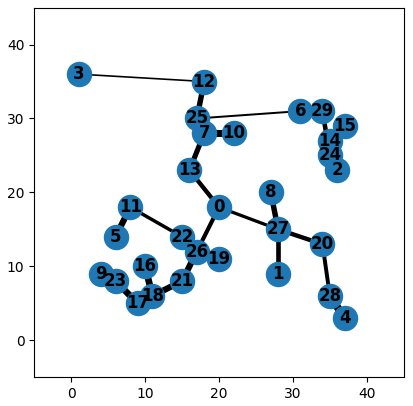
\includegraphics[width=0.33\columnwidth]{figures/RandomLayout.png}
\end{center}
\caption{Randomly distributed network of 30 nodes connected with an opportunistic protocol. Weight of the line indicates the connection latency or distance between nodes.}
\label{fig:randomnetwork}
\end{figure}
\begin{figure}
\begin{center}
\includegraphics[width=0.33\columnwidth]{figures/MasterLayout.png}
\end{center}
\caption{Circular network utilizing a master node at the center.}
\label{fig:circularnetwork}
\end{figure}
\begin{figure}
\begin{center}
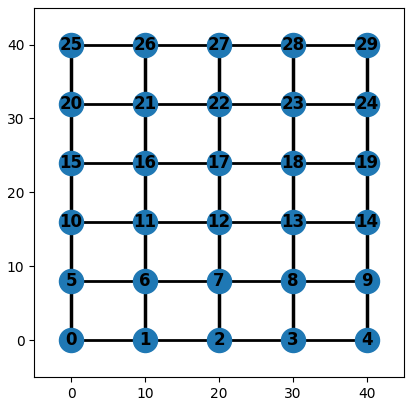
\includegraphics[width=0.33\columnwidth]{figures/GridLayout.png}
\end{center}
\caption{Grid network with only adjacent vertical and horizontal connections to nearest neighbors.}
\label{fig:gridnetwork}
\end{figure}

\subsection{Damaging the network}
Next an array of randomly damaged networks had to be created to be run through the function that would determine the network architectures. A function was created that took and undamaged network as an argument and randomly removed five of its nodes and all connections to or from those nodes. This produced the damaged networks (examples shown in \fref{fig:damagerandom}, \fref{fig:damagecircular}, \fref{fig:damagegrid}) that would be used in the simulation.
\begin{figure}
\begin{center}
\includegraphics[width=0.33\columnwidth]{figures/DamagedRandomLayout.png}
\end{center}
\caption{Damaged random network.}
\label{fig:damagerandom}
\end{figure}
\begin{figure}
\begin{center}
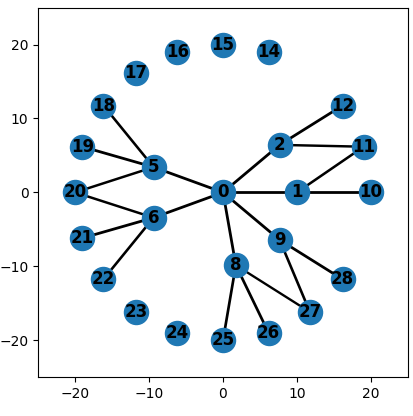
\includegraphics[width=0.33\columnwidth]{figures/DamagedMasterLayout.png}
\end{center}
\caption{Damaged master network.}
\label{fig:damagecircular}
\end{figure}
\begin{figure}
\begin{center}
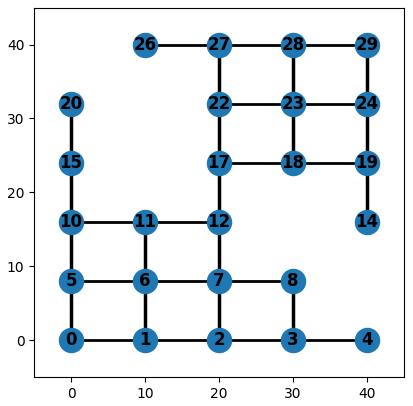
\includegraphics[width=0.33\columnwidth]{figures/DamagedGridLayout.png}
\end{center}
\caption{Damaged grid network.}
\label{fig:damagegrid}
\end{figure}

\subsection{Monte Carlo sampling method}
To test the damaged networks, the simulation ran 1000 iterations of collecting the average survivability rate and the surviving path length from 100 randomly damaged networks. Using an average velocity of sound in saltwater of $c=\SI{1510}{\meter\per\second}$, the average travel latency of the acoustic signal was calculated from the average path length. A convergence check was carried out by running the simulation once for 10,000 iterations (rates did not change appreciably). 

\subsection{Code}
The following pseudocode provides a basic overview of how the code tests the survivability of various mesh network layouts. The actual Python source code to generate networks is avaiialble at \url{https://github.com/Stites-2021/Network-Layouts}. The Python source code for survivability analyses is available at \url{https://github.com/Stites-2021/Survivability}.  
\lstset{basicstyle=\ttfamily\scriptsize}
\begin{lstlisting}
Define Create_Network_Function()
	return desired_network_layout
Define Delete_Nodes_Function(Network)
	i = 0
	while 1=<5
		delete random node in Network 
		i=i+1
	return damaged_network
Define Find_Survivability/Latency_Function(Damaged_Network)
	i = 0
	while 1=<100
		Pick two random nodes in Damaged_Network
		Find if path exists or not between them
		If path exists find the length
		i = i+1
	Survivability = Find ratio of successful connections to... 
	total connection attempts
	Path_Length = Find average surviving path length
	return [Survivability, Path_Length]
i = 0
while 1=<1000
	Network = Create_Network_Function()
	Damaged_Network = Delete_Nodes_Function(Network)
	[Survivability[i], Path_Length[i]]...
	= Find_Survivability/Latency_Function(Damaged_Network)
	i = i+1
Final_Values = Average([Survivability, Path_Length])
\end{lstlisting}







\clearpage
\section{Results}

\Fref{tab:results} shows the simulation results (survivability rate $p$ and surviving path length $\lambda$) for the three different network architectures (random, circular-master, and grid).  

\begin{table}[h]
\caption{A table showing the simulation results for each network type.}
\label{tab:results}
\begin{center}
%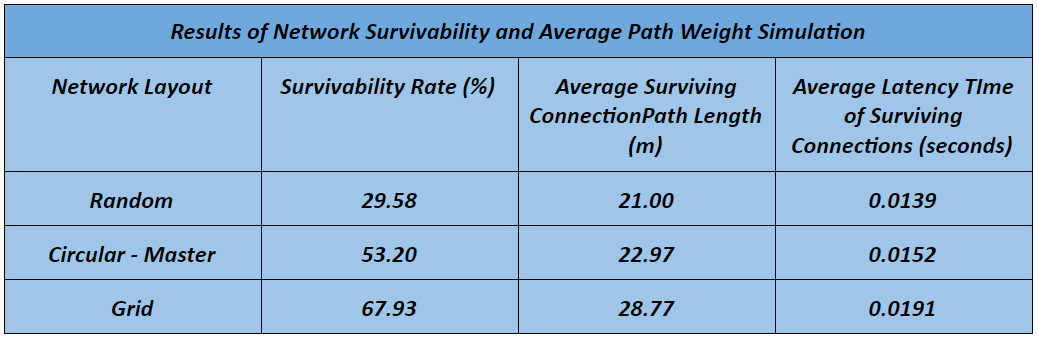
\includegraphics[width=0.6\columnwidth]{tables/ResultsTable.PNG}
  \begin{tabularx}{\columnwidth}{p{0.75in}p{0.75in}p{0.75in}p{0.75in}}
    \toprule
    network layout & survivability rate (\si{\percent}) & {\raggedright average surviving connection path length (\si{\meter})} & {\raggedright average travel latency time of surviving connections (\si{\second})}\\
    \midrule
    random & 25.98 & 21.00 & 0.0139\\
    circular-master & 53.20 & 22.97 & 0.0152 \\
    grid & 67.93 & 28.77 & 0.0191 \\
    \bottomrule
    \end{tabularx}
\end{center}
\end{table}

To examine the distribution and spread of survivability rate ($p$) and surviving path length ($\lambda$), I plotted histograms of the data from 1000 replicates. These are shown in \fref{fig:historandom}, \fref{fig:histomaster}, and \fref{fig:histogrid}.  
\begin{figure}[h]
\begin{center}
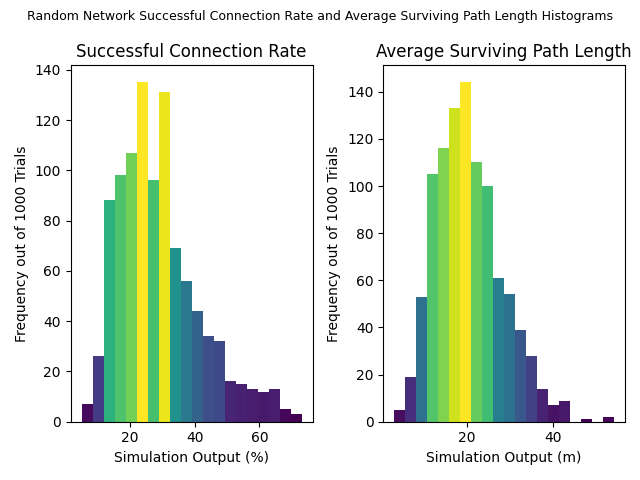
\includegraphics[width=\columnwidth]{figures/RandomHistogram.png}
\end{center}
\caption{A histogram showing the simulation result distribution for the random network.}
\label{fig:historandom}
\end{figure}
\begin{figure}[h]
\begin{center}
\includegraphics[width=\columnwidth]{figures/MasterHistogram.png}
\end{center}
\caption{A histogram showing the simulation result distribution for the master network.}
\label{fig:histomaster}
\end{figure}
\begin{figure}[h]
\begin{center}
\includegraphics[width=\columnwidth]{figures/GridHistogram.png}
\end{center}
\caption{A histogram showing the simulation result distribution for grid network.}
\label{fig:histogrid}
\end{figure}

\section{Discussion}
\subsection{Clear differences between network architectures}
The results of the simulation showed that the random network performed least well over both aspects of the simulation (\fref{tab:results}, \fref{fig:historandom}). This result was expected as the random network was intended mostly as null model and basis for comparison. 

The master network demonstrated the lowest surviving connection path length, and consequently, the lowest acoustic signal travel latency (\fref{tab:results}, \fref{fig:histomaster}).  This is due to the circular arrangement allowing pseudo-diagonal connections across the testing area compared to the grid network’s vertical and horizontally aligned connections. 

In terms of survivability however, the grid network’s repetitive communication architecture proved to have superior redundancy over the master network (\fref{tab:results}, \fref{fig:histogrid}). This is due to the fact that the master network is heavily reliant on the master node for its connection architecture as it it is the only path between the inner circle of worker nodes. If the master nod is removed, the network is very vulnerable to connection failure.  

\subsection{Which is ``best''?}
The results of the simulation show that a circularly arranged master node network has advantages in terms of reducing travel latency while a grid network provides an advantage in survivability. A user could choose between these networks based on the perceived threat to the network and/or desired transmission speed within the network. A single network could also be designed to incorporate aspects from both  (including diagonal connections in the grid algorithm for example) in order to combine the strengths of the two networks. While the results of this simulation were not particularly surprising, the process of building the networks and simulations laid the groundwork for deeper research questions that will be explored next semester regarding additional network spatial arrangements as well as more advanced routing protocols and network healing algorithms.

\subsection{A tool for moving forward}
I was able to evaluate different network architectures for a 30-node network over a small area. The tool was able to examine various metrics of robustness to damage and transmission time. Moving forward, I plan to evaluate other metrics and extend the simulation for various scenarios of interest. 

%Using the metrics of transmission time (given by the transmission’s latency), successful transmission rate (given by the transmission’s throughput and packet loss rates), and immunity to node failure I will evaluate different architectures of a 20 node mesh network. This will be done using simulation, probably through MATLAB software and Python based NetworkX software \cite{hagberg2008exploring}. The network simulation C++ based software NS-3 has also been shown to be highly successful at modeling UDP transmission based mesh networks and could be used \cite{dugaev2020wireless}. Using these software platforms, different processes could be coded and simulated and the above metrics could be measured and evaluated.

\section*{Acknowledgements}
I acknowledge the support of the Frank L.~Bowman Scholarship Program at the United States Naval Academy. 

\bibliography{IEEEabrv, stites.bib}

\begin{IEEEbiography}[{\includegraphics[width=1in,height=1.25in,clip,keepaspectratio]{\myroot/figures/M216468.jpg}}]{Corwin Wesley Stites} is a midshipman at the United States Naval Academy majoring in Robotics and Control Engineering. Stites is a Bowman Scholar at USNA; upon graduation, he hopes to attend graduate school, after which he will serve as a submarine officer. He enjoys applying to graduateschool, German, and Python coding. 
\end{IEEEbiography}
\end{document}


% Copied from poster by DE
%\section*{Introduction}
%Underwater surveying is a costly and time consuming endeavor. Large areas of ocean must have bathymetry data regularly updated in order to allow for safe ship navigation. Furthermore, finding a submerged target such as a wreckage or explosive device  requires large areas of ocean to be surveyed. Unmanned Underwater Vehicles have proven success in greatly streamlining the hydrographic surveying process by allowing for collaborative fleet surveying. Creating a mobile network of UUVs provides opportunities for further autonomization of hydrographic surveying.  A mesh network made up of UUVs acting a sindividual nodes would allow for collaborative position and velocity tracking within the network  thus  removing the need for constant shipboard control. When designing such a network, redundancy in the network will be a critical aspect of the design. In other words, the network must be able to route around missing nodes in the event that a UUV is damaged or goes offline.
%\begin{figure}
%\begin{center}
%image here
%\end{center}
%\caption{An example of fleet UUV network technology. Ocean Infinity Hugin AUVs conducting hydrographic surveying while being controlled by a ship mounted acoustic modem.}
%\end{figure}
%
%\subsection*{Problem statement}
%The aim of this research was to investigate the redundancy of different UUV mesh networks built for the purpose of conducting hydrographic surveying. The research determined how the spatial arrangement of nodes in a network and the connection architecture of the network would affect the ability of a network to function in the event of multiple offline nodes. Three types of network spatial arrangements were investigated each with a different connection architecture protocol. 
%\begin{enumerate}
%\item A network of randomly distributed nodes using an opportunistic connection algorithm (connection formed between closest nodes). 
%\item A network made up of a ``master node'' surrounded by two concentric circles of worker nodes connected by a branching algorithm.
%\item A grid network connected by a grid algorithm. 
%\end{enumerate}
%
%\section*{Methods and materials}
%The method of testing was software simulation. The code was written in Python utilizing the \lstinline{networkx} library to build and simulate the networks. A few key control variables were set during the tests.
%\begin{enumerate}
%\item All networks were arranged in a \SI{40}{\meter\squared} operating area.
%\item All networks were built with 30 nodes.
%\item 5 nodes were removed from each network to simulate a damaged network.
%\end{enumerate}
%The simulation ran 1000 iterations of collecting the average survivability (successful connection rate between two random nodes) and the average surviving connection length from 100 randomly damaged networks. Using an average speed of sound in saltwater of  $V_{sound} = \SI{1510}{\meter\per\second}$, the average travel latency of the acoustic signal was calculated from the path length.
%
%\begin{figure}
%\begin{center}
%Code block here
%\end{center}
%\caption{Pseudocode providing a basic synopsis of the simulation code}
%\end{figure}
%
%\begin{figure}
%\begin{center}
%image here
%\end{center}
%\caption{NetworkX Plots showing from left to right a randomly distributed network, a circular master node network, and a grid network.}
%\end{figure}
%
%\begin{figure}
%\begin{center}
%image here
%\end{center}
%\caption{NetworkX Plots showing the above networks after having been run through a function to randomly remove five nodes.}
%\end{figure}
%
%\section*{Results}
%\begin{table}
%\caption{Table of simulation outputs. Results of network sensitivity and average path weight simulation.}
%\begin{center}
%  \begin{tabular}{cccc}
%    \toprule
%    network layout & survivability rate (\si{\percent}) & average surviving connection path length (\si{\meter}) & average travel latency time of surviving connections (\si{\second})\\
%    \midrule
%    random & 25.98 & 21.00 & 0.0139\\
%    circular-master & 53.20 & 22.97 & 0.0152 \\
%    grid & 67.93 & 28.77 & 0.0191 \\
%    \bottomrule
%    \end{tabular}
%\end{center}
%\end{table}
%
%\begin{figure}
%\begin{center}
%image here
%\end{center}
%\caption{Histograms showing the frequency of successful connection rates and average surviving path lengths out of 1000 trials for each graph type.}
%\end{figure}
%
%\section{Discussion}
%\begin{block}{Discussion}
%The results of the simulation showed that the random network performed least well over both aspects of the simulation. This result was expected as the random network was intended mostly as a basis for comparison. The master network demonstrated the lowest surviving connection path length, and consequently, the lowest acoustic signal travel latency.  This is due to the circular arrangement allowing pseudo-diagonal connections across the testing area compared to the grid networks vertical and horizontally aligned connections. In terms of survivability however, the grid networks repetitive communication architecture proved to have superior redundancy over the master network. 
%
%The results of the simulation show that a circularly arranged master node network has advantages in terms of reducing travel latency while a grid network provides an advantage in survivability. A user could choose between these networks based on the perceived threat to the network and/or the user’s desired network transmission speed within the network. One network could also be designed to incorporate aspects from the other (including diagonal connections in the grid algorithm for example) in order to combine the strengths of the two networks. While the results of this simulation were not particularly surprising, the process of building the networks and simulations laid the groundwork for deeper research questions that will be explored next semester regarding additional network spatial arrangements as well as more advanced routing protocols and network healing algorithms.
%
%\section*{Acknowledgements}
%
%%\section*{References}
%%\begin{block}{References}
%%\bibliographystyle{IEEEtrans} % or IEEEtrans if you want that kind
%%\scriptsize\bibliography{poster.bib}
%%\end{block}
%
